\documentclass{standalone}
\usepackage{tikz}
\usetikzlibrary{patterns, positioning}


\begin{document}
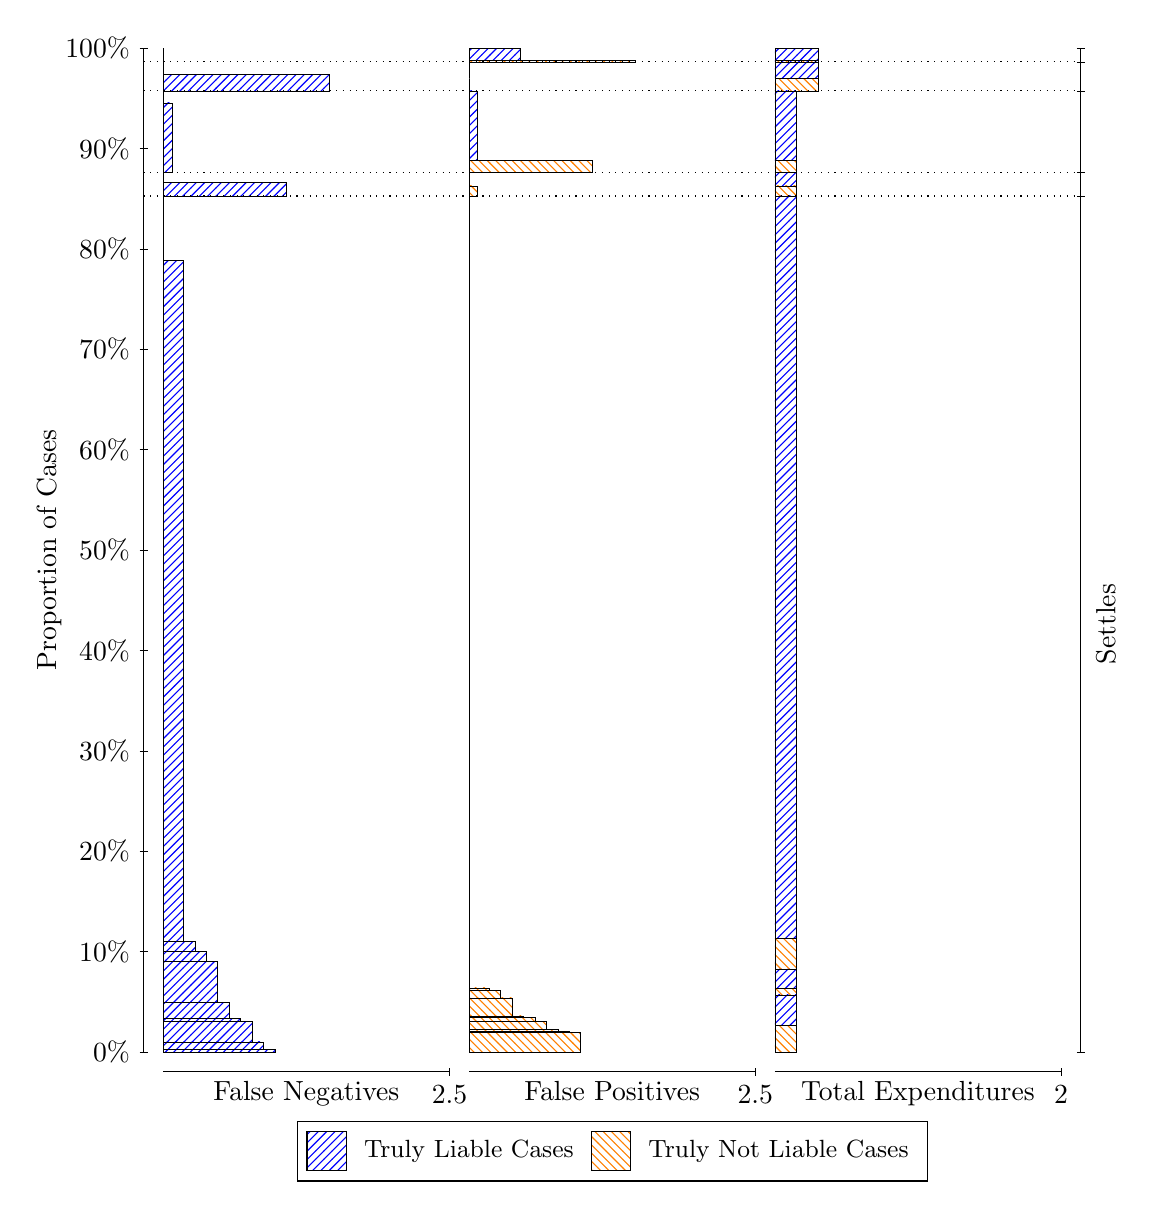
\begin{tikzpicture}
\draw[black, very thin] (1.5,1.75) -- (1.5,14.5);
\node[rotate=90, text=black, anchor=center] at (0.3, 8.125) {Proportion of Cases};
\draw[black, very thin] (1.45,1.75) -- (1.55,1.75);
\node[text=black, anchor=east] at (1.45, 1.75) {0\%};
\draw[black, very thin] (1.45,3.025) -- (1.55,3.025);
\node[text=black, anchor=east] at (1.45, 3.025) {10\%};
\draw[black, very thin] (1.45,4.3) -- (1.55,4.3);
\node[text=black, anchor=east] at (1.45, 4.3) {20\%};
\draw[black, very thin] (1.45,5.575) -- (1.55,5.575);
\node[text=black, anchor=east] at (1.45, 5.575) {30\%};
\draw[black, very thin] (1.45,6.85) -- (1.55,6.85);
\node[text=black, anchor=east] at (1.45, 6.85) {40\%};
\draw[black, very thin] (1.45,8.125) -- (1.55,8.125);
\node[text=black, anchor=east] at (1.45, 8.125) {50\%};
\draw[black, very thin] (1.45,9.4) -- (1.55,9.4);
\node[text=black, anchor=east] at (1.45, 9.4) {60\%};
\draw[black, very thin] (1.45,10.675) -- (1.55,10.675);
\node[text=black, anchor=east] at (1.45, 10.675) {70\%};
\draw[black, very thin] (1.45,11.95) -- (1.55,11.95);
\node[text=black, anchor=east] at (1.45, 11.95) {80\%};
\draw[black, very thin] (1.45,13.225) -- (1.55,13.225);
\node[text=black, anchor=east] at (1.45, 13.225) {90\%};
\draw[black, very thin] (1.45,14.5) -- (1.55,14.5);
\node[text=black, anchor=east] at (1.45, 14.5) {100\%};

\draw[black, very thin] (13.4,1.75) -- (13.4,14.5);
\draw[black, very thin] (13.35,1.75) -- (13.45,1.75);
\node[anchor=west] at (13.35, 1.75) {};
\draw[black, very thin] (13.35,12.621) -- (13.45,12.621);
\node[anchor=west] at (13.35, 12.621) {};
\draw[black, very thin] (13.35,12.92) -- (13.45,12.92);
\node[anchor=west] at (13.35, 12.92) {};
\draw[black, very thin] (13.35,13.957) -- (13.45,13.957);
\node[anchor=west] at (13.35, 13.957) {};
\draw[black, very thin] (13.35,14.324) -- (13.45,14.324);
\node[anchor=west] at (13.35, 14.324) {};
\draw[black, very thin] (13.35,14.5) -- (13.45,14.5);
\node[anchor=west] at (13.35, 14.5) {};

\draw[black, very thin, pattern color=blue, pattern=north east lines] (1.75,1.75) rectangle (3.167,1.7874);
\draw[black, very thin, pattern color=blue, pattern=north east lines] (1.75,1.7874) rectangle (3.0217,1.8793);
\draw[black, very thin, pattern color=blue, pattern=north east lines] (1.75,1.8793) rectangle (2.8763,2.1431);
\draw[black, very thin, pattern color=blue, pattern=north east lines] (1.75,2.1431) rectangle (2.731,2.1741);
\draw[black, very thin, pattern color=blue, pattern=north east lines] (1.75,2.1741) rectangle (2.5857,2.3791);
\draw[black, very thin, pattern color=blue, pattern=north east lines] (1.75,2.3791) rectangle (2.4403,2.9009);
\draw[black, very thin, pattern color=blue, pattern=north east lines] (1.75,2.9009) rectangle (2.295,3.0311);
\draw[black, very thin, pattern color=blue, pattern=north east lines] (1.75,3.0311) rectangle (2.1497,3.158);
\draw[black, very thin, pattern color=blue, pattern=north east lines] (1.75,3.158) rectangle (2.0043,11.806);
\draw[black, very thin, pattern color=orange, pattern=north west lines] (1.75,11.806) rectangle (1.75,12.621);
\draw[black, very thin, pattern color=blue, pattern=north east lines] (1.75,12.621) rectangle (3.3123,12.791);
\draw[black, very thin, pattern color=orange, pattern=north west lines] (1.75,12.791) rectangle (1.75,12.92);
\draw[black, very thin, pattern color=blue, pattern=north east lines] (1.75,12.92) rectangle (1.859,13.803);
\draw[black, very thin, pattern color=orange, pattern=north west lines] (1.75,13.803) rectangle (1.75,13.957);
\draw[black, very thin, pattern color=blue, pattern=north east lines] (1.75,13.957) rectangle (3.8573,14.169);
\draw[black, very thin, pattern color=orange, pattern=north west lines] (1.75,14.169) rectangle (1.75,14.324);
\draw[black, very thin, pattern color=orange, pattern=north west lines] (1.75,14.324) rectangle (1.75,14.347);
\draw[black, very thin, pattern color=blue, pattern=north east lines] (1.75,14.347) rectangle (1.75,14.5);
\draw[black, very thin, pattern color=orange, pattern=north west lines] (5.6333,1.75) rectangle (7.0503,1.9947);
\draw[black, very thin, pattern color=orange, pattern=north west lines] (5.6333,1.9947) rectangle (6.905,2.0141);
\draw[black, very thin, pattern color=orange, pattern=north west lines] (5.6333,2.0141) rectangle (6.7597,2.0354);
\draw[black, very thin, pattern color=orange, pattern=north west lines] (5.6333,2.0354) rectangle (6.6143,2.1395);
\draw[black, very thin, pattern color=orange, pattern=north west lines] (5.6333,2.1395) rectangle (6.469,2.1918);
\draw[black, very thin, pattern color=orange, pattern=north west lines] (5.6333,2.1918) rectangle (6.3237,2.2042);
\draw[black, very thin, pattern color=orange, pattern=north west lines] (5.6333,2.2042) rectangle (6.3237,2.2093);
\draw[black, very thin, pattern color=orange, pattern=north west lines] (5.6333,2.2093) rectangle (6.1783,2.4365);
\draw[black, very thin, pattern color=orange, pattern=north west lines] (5.6333,2.4365) rectangle (6.033,2.5289);
\draw[black, very thin, pattern color=orange, pattern=north west lines] (5.6333,2.5289) rectangle (5.8877,2.5647);
\draw[black, very thin, pattern color=blue, pattern=north east lines] (5.6333,2.5647) rectangle (5.6333,12.621);
\draw[black, very thin, pattern color=orange, pattern=north west lines] (5.6333,12.621) rectangle (5.7423,12.75);
\draw[black, very thin, pattern color=blue, pattern=north east lines] (5.6333,12.75) rectangle (5.6333,12.92);
\draw[black, very thin, pattern color=orange, pattern=north west lines] (5.6333,12.92) rectangle (7.1957,13.074);
\draw[black, very thin, pattern color=blue, pattern=north east lines] (5.6333,13.074) rectangle (5.7423,13.957);
\draw[black, very thin, pattern color=orange, pattern=north west lines] (5.6333,13.957) rectangle (5.6333,14.111);
\draw[black, very thin, pattern color=blue, pattern=north east lines] (5.6333,14.111) rectangle (5.6333,14.324);
\draw[black, very thin, pattern color=orange, pattern=north west lines] (5.6333,14.324) rectangle (7.7407,14.347);
\draw[black, very thin, pattern color=blue, pattern=north east lines] (5.6333,14.347) rectangle (6.2873,14.5);
\draw[black, very thin, pattern color=orange, pattern=north west lines] (9.5167,1.75) rectangle (9.7892,2.0871);
\draw[black, very thin, pattern color=blue, pattern=north east lines] (9.5167,2.0871) rectangle (9.7892,2.4738);
\draw[black, very thin, pattern color=orange, pattern=north west lines] (9.5167,2.4738) rectangle (9.7892,2.5619);
\draw[black, very thin, pattern color=blue, pattern=north east lines] (9.5167,2.5619) rectangle (9.7892,2.8043);
\draw[black, very thin, pattern color=orange, pattern=north west lines] (9.5167,2.8043) rectangle (9.7892,3.1938);
\draw[black, very thin, pattern color=blue, pattern=north east lines] (9.5167,3.1938) rectangle (9.7892,12.621);
\draw[black, very thin, pattern color=orange, pattern=north west lines] (9.5167,12.621) rectangle (9.7892,12.75);
\draw[black, very thin, pattern color=blue, pattern=north east lines] (9.5167,12.75) rectangle (9.7892,12.92);
\draw[black, very thin, pattern color=orange, pattern=north west lines] (9.5167,12.92) rectangle (9.7892,13.074);
\draw[black, very thin, pattern color=blue, pattern=north east lines] (9.5167,13.074) rectangle (9.7892,13.957);
\draw[black, very thin, pattern color=orange, pattern=north west lines] (9.5167,13.957) rectangle (10.062,14.111);
\draw[black, very thin, pattern color=blue, pattern=north east lines] (9.5167,14.111) rectangle (10.062,14.324);
\draw[black, very thin, pattern color=orange, pattern=north west lines] (9.5167,14.324) rectangle (10.062,14.347);
\draw[black, very thin, pattern color=blue, pattern=north east lines] (9.5167,14.347) rectangle (10.062,14.5);
\draw[black, dotted] (1.5,12.621) -- (13.4,12.621);
\draw[black, dotted] (1.5,12.92) -- (13.4,12.92);
\draw[black, dotted] (1.5,13.957) -- (13.4,13.957);
\draw[black, dotted] (1.5,14.324) -- (13.4,14.324);
\draw[black, very thin] (1.75,1.5) -- (5.3833,1.5);
\node[text=black, anchor=north] at (3.5667, 1.5) {False Negatives};
\draw[black, very thin] (5.3833,1.45) -- (5.3833,1.55);
\node[text=black, anchor=north] at (5.3833, 1.45) {2.5};

\draw[black, very thin] (5.6333,1.5) -- (9.2667,1.5);
\node[text=black, anchor=north] at (7.45, 1.5) {False Positives};
\draw[black, very thin] (9.2667,1.45) -- (9.2667,1.55);
\node[text=black, anchor=north] at (9.2667, 1.45) {2.5};

\draw[black, very thin] (9.5167,1.5) -- (13.15,1.5);
\node[text=black, anchor=north] at (11.333, 1.5) {Total Expenditures};
\draw[black, very thin] (13.15,1.45) -- (13.15,1.55);
\node[text=black, anchor=north] at (13.15, 1.45) {2};

\node[text=black, centered, rotate=90] at (13.72, 7.1854) {Settles};





\draw (7.449999999999999,1.5) node[draw=none] (baseCoordinate) {};
\begin{scope}[align=center]
        \matrix[scale=0.5, draw=black, below=0.5cm of baseCoordinate, nodes={draw}, column sep=0.1cm]{
            \node[rectangle, draw, minimum width=0.5cm, minimum height=0.5cm, pattern color=blue, pattern=north east lines] {}; &
            \node[draw=none, font=\small, text=black] (B) {Truly Liable Cases}; &
            \node[rectangle, draw, minimum width=0.5cm, minimum height=0.5cm, pattern color=orange, pattern=north west lines] {}; &
            \node[draw=none, font=\small, text=black] (B) {Truly Not Liable Cases}; \\
            };
\end{scope}

\end{tikzpicture}
\end{document}